\documentclass[tikz,border=3mm]{standalone}
\usepackage{pgfplots}
\pgfplotsset{compat=1.17}
\usepgfplotslibrary{groupplots}
\usetikzlibrary{arrows.meta,positioning,fit,shapes.geometric,calc,backgrounds}
\begin{document}

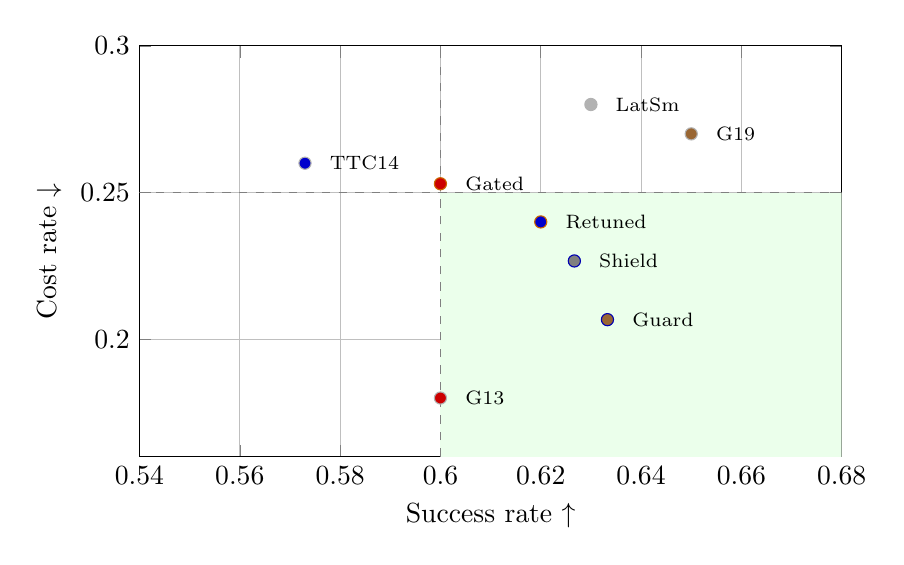
\begin{tikzpicture}
\begin{axis}[width=10.5cm,height=6.8cm,xlabel={Success rate $\uparrow$},ylabel={Cost rate $\downarrow$},xmin=0.54,xmax=0.68,ymin=0.16,ymax=0.30,grid=major]
\fill[green!8] (axis cs:0.60,0.16) rectangle (axis cs:0.68,0.25);
\draw[dashed, gray] (axis cs:0.60,0.16)--(axis cs:0.60,0.30);
\draw[dashed, gray] (axis cs:0.54,0.25)--(axis cs:0.68,0.25);
\addplot+[only marks, mark=*, mark size=2.2pt, color=gray!60] coordinates {(0.5730,0.2600)};
\node[font=\scriptsize, anchor=west] at (axis cs:0.5760,0.2600) {TTC14};
\addplot+[only marks, mark=*, mark size=2.2pt, color=gray!60] coordinates {(0.6000,0.1800)};
\node[font=\scriptsize, anchor=west] at (axis cs:0.6030,0.1800) {G13};
\addplot+[only marks, mark=*, mark size=2.2pt, color=gray!60] coordinates {(0.6500,0.2700)};
\node[font=\scriptsize, anchor=west] at (axis cs:0.6530,0.2700) {G19};
\addplot+[only marks, mark=*, mark size=2.2pt, color=gray!60] coordinates {(0.6300,0.2800)};
\node[font=\scriptsize, anchor=west] at (axis cs:0.6330,0.2800) {LatSm};
\addplot+[only marks, mark=*, mark size=2.2pt, color=orange!80!black] coordinates {(0.6200,0.2400)};
\node[font=\scriptsize, anchor=west] at (axis cs:0.6230,0.2400) {Retuned};
\addplot+[only marks, mark=*, mark size=2.2pt, color=orange!80!black] coordinates {(0.6000,0.2530)};
\node[font=\scriptsize, anchor=west] at (axis cs:0.6030,0.2530) {Gated};
\addplot+[only marks, mark=*, mark size=2.2pt, color=blue!70!black] coordinates {(0.6333,0.2067)};
\node[font=\scriptsize, anchor=west] at (axis cs:0.6363,0.2067) {Guard};
\addplot+[only marks, mark=*, mark size=2.2pt, color=blue!70!black] coordinates {(0.6267,0.2267)};
\node[font=\scriptsize, anchor=west] at (axis cs:0.6297,0.2267) {Shield};
\end{axis}
\end{tikzpicture}

\end{document}
